\chapter{The framework}

\section{Main Scenario}

The goal is to build a platform that allows a user to query for experts in a particular domain. The
platform extracts and unifies the required information from a variety of online sources and
subsequently builds a repository of user profiles. We basically want to create a framework that would function as a Google for finding experts given a certain subject.

We will use the following steps to build such a platform:

%verduidelijken dat de volgorde van deze stappen niet belangrijk is, ze zijn interchangeable

\begin{itemize}
	%Welke auteur namen ? Waar halen we die vandaan ? Conference sites ?
	\item \textbf{Seed data} We need a list of author names to start with.
	\item \textbf{Information extraction}
		\begin{itemize}
			\item Looking up personal information, ie. profiles from LinkedIn.
			\item Looking up publications, extracting title, co-authors and affiliation. The co-authors can be used as new input for further information extraction.
			\item Categorize publications by subject
		\end{itemize}
	\item \textbf{Disambiguation} Decide if there are different authors with the same name or different spellings of the same author's name which should be mapped to one author.
\end{itemize}

%Describe how we got to the architecture for the framework, show a figure of the (simplified + extensive) architecture and explain the different components.

\section{Features}

We need to extract information. We need seed data which we can use to start this process. We need data which we can link to this seed data. We need sites or databases where we can find this data. As data we need publication titles, author names, affiliations, abstracts, keywords, publication text, author profiles, email adresses, subjects ... We will write plugins, each dedicated to one source which will be used to add extra information to the database, connected to existing data, in some way.



\subsection{Information extraction}

We want to create a framework that can search different online sources autonomously and extract information. We 


\subsection{Information linkage}



\subsection{Pitfalls}

Describe the possible difficulties: people with the same name that are a different person, a person who's name is written differently (usage of abbreviations, altering last name due to marriage...), change of expertise due to change of interest/job.

\section{Components / Architecture}

\begin{figure}[htbp]
	\centering
		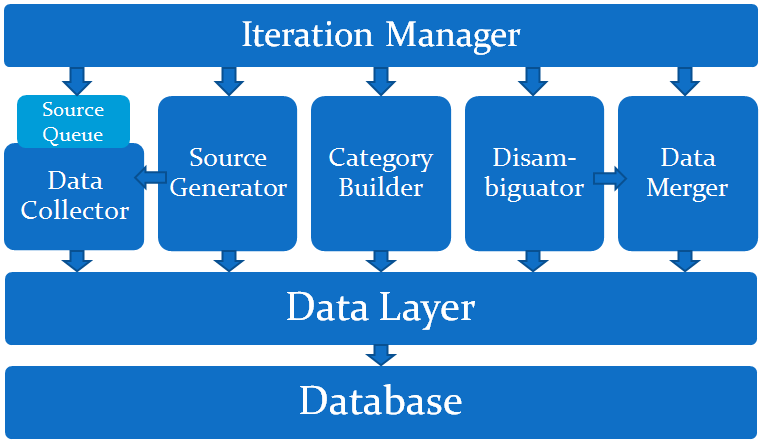
\includegraphics[width=1.00\textwidth]{fig/architectuur.png}
	\caption{First attempt at the architecture based on the necessary components}
	\label{fig:architectuur}
\end{figure}

Plugins, IterationManager, CategoryBuilder, Disambiguator, DataMerger

\section{Technologies}

\subsection{MySQL}

Discuss the differences, advantages and disadvantages between a relational datastore, a record-store and a triple-store.

\subsubsection{Relational datastore}

\subsubsection{A record-store}

\subsubsection{Triple-store}

\subsubsection{Conclusion}

We choose to use MySQL, a relational datastore, because we are familiar with it. It allows us to quickly set up our prototype to work and test our framework on.

\subsection{Two databases}

We use two databases, one for development and one for production.

The former is used to collect all information about the possible experts and their work. 

\subsection{Ruby}
